% ============================================================
%  SECTION 1 — INTRODUCTION
% ============================================================

% ------------------------------------------------------------
\subsection{Motivation and Problem Context}
\label{subsec:motivation}
% ------------------------------------------------------------

Large infrastructure and engineering projects routinely overrun their budgets
and miss their schedules \citep{Flyvbjerg2003, Merrow2011}. When a portfolio
of such projects executes simultaneously under a shared capital commitment,
the risks compound: a performance shortfall on one project propagates through
the shared budget to all others, and the decision of how much to allocate to
each project at each period can determine whether the portfolio succeeds or fails.

Despite this, the formal treatment of portfolio-level budget allocation as a
sequential decision problem is absent from the project portfolio management
literature. Research has concentrated on the \emph{selection} stage --- which
projects to include --- while the \emph{operational governance} stage --- how
to manage a committed portfolio through to completion --- has received
comparatively little analytical treatment \citep{Archer1999, Cooper2001,
Turner2014}. The present work fills this gap by delivering a verified simulation environment
that makes the problem tractable for data-driven methods and establishing a
performance baseline that quantifies the cost of naive allocation.

We consider a portfolio of $n$ projects, each governed by a bilateral contract
consistent with FIDIC forms \citep{FIDIC2017}, executing concurrently under a
relaxed capital commitment. A portfolio manager exercises one recurring
decision at each discrete planning period: how much budget to allocate to each
active project. The formal problem is to find the allocation policy that
maximises discounted net cash flow across the portfolio horizon while
respecting contract mechanics.

% ------------------------------------------------------------
\subsection{The Project Management Decision Hierarchy}
\label{subsec:hierarchy}
% ------------------------------------------------------------

The present contribution operates at the portfolio governance layer of the
three-tier project management hierarchy \citep{PMI2017}. Portfolio selection
--- which projects to commit to --- is treated as an exogenous input,
consistent with the two-stage governance model of \citet{Turner2014}.
At the governance layer, the portfolio manager does not control project
execution directly but allocates budget to each project and observes
earned value outcomes. Termination is not a deliberate agent action but 
an endogenous environment mechanic. It is triggered by one of two independent 
conditions. The first is a hard deadline: if the current episode timestep reaches 
planned finish + finish delay cap, the project is terminated immediately regardless 
of progress or tolerance. The second is sustained underperformance: if a project’s 
actual progress falls behind its planned progress by more than progress delay cap, 
a tolerance counter decrements by one each period the breach persists and resets to 
its initial value whenever the breach clears; termination fires when the counter reaches zero. 

Project termination differs from episode termination — a project terminates individually 
and triggers a settlement cash flow, while the episode ends only when every project has 
either completed or been terminated, or when the global horizon is reached, or when the 
portfolio budget is exhausted with no pending inflows.

\begin{figure}[H]
  \centering
  \resizebox{\textwidth}{!}{%
  \begin{tikzpicture}[
    every node/.style = {font=\normalsize},
    box/.style = {
      rectangle, rounded corners=6pt,
      draw, thick,
      minimum width=3.4cm, minimum height=1.2cm,
      align=center
    },
    agent/.style  = {box, draw=violet!70!black, fill=violet!10},
    contr/.style  = {box, draw=orange!70!red,   fill=orange!8},
    client/.style = {box, draw=teal!70!black,   fill=teal!8},
    state/.style  = {
      rectangle, rounded corners=6pt,
      draw=gray!60, thick, fill=gray!6,
      minimum width=17cm, minimum height=1.3cm,
      align=center
    },
    act/.style  = {-{Latex[length=6pt]}, thick, violet!70!black},
    rew/.style  = {-{Latex[length=6pt]}, thick, blue!60!black, dashed},
    obs/.style  = {-{Latex[length=6pt]}, thick, gray!50!black},
    prog/.style = {-{Latex[length=6pt]}, thick, orange!70!red},
    int/.style  = {-{Latex[length=6pt]}, thick, teal!60!black, dashed},
    lbl/.style  = {font=\normalsize},
  ]

    \node[agent] (pm) {%
      \textbf{Portfolio Manager}\\[2pt]
      policy $\pi(S_t)\!\to\!\mathbf{x}_t$};

    \node[client, right=10cm of pm] (client) {%
      \textbf{Client}\\[2pt]
      milestone approval};

    \node[contr, left=3cm of client] (contractor) {%
      \textbf{Contractor}\\[2pt]
      project execution};

    \node[
      rectangle, rounded corners=20pt,
      draw=orange!50!black, thick, fill=orange!4,
      inner xsep=20pt, inner ysep=18pt,
      fit=(contractor)(client),
      label={[font=\footnotesize\itshape, text=orange!60!black]
             above:Environment \textit{(contract)}},
    ] (env) {};

    \node[client, right=10cm of pm] (client) {%
      \textbf{Client}\\[2pt]
      milestone approval};

    \node[contr, left=3cm of client] (contractor) {%
      \textbf{Contractor}\\[2pt]
      project execution};

    \node[state,
          below=3.5cm of $(pm.south)!0.55!(contractor.south)$] (state)
          {\textbf{Observable State} $S_t$:\quad
          $\bigl\{\tau_{i,t}^{\mathrm{rem}},\;
          \mathrm{ca}_{i,t}/B_0,\;
          \mathrm{ca}_{i,t+1}/B_0,\;
          \Delta p_{i,t}^{\mathrm{gap}},\;
          \Delta t_{i,t}^{\mathrm{gap}}/H,\;
          \mathrm{ar}_{i,t}/B_0,\;
          \widetilde{\mathrm{NPV}}_{i,t}\bigr\}_{i},\;
          \mathrm{ncf}_t/B_0,\;B_t/B_0$};

    \draw[act]
      (pm.east) -- (contractor.west)
      node[midway, above, lbl, violet!80!black] {allocation $\mathbf{x}_t$};

    \draw[prog]
      (contractor.east) -- (client.west)
      node[midway, above, lbl, orange!80!red] {progress $\Delta P_{i,t}$};

    \draw[rew]
      (client.north)
        -- ++(0, 1.4)
        -| (pm.north)
      node[pos=0.28, above, lbl, blue!60!black]
        {$r_t = \gamma^t(\mathrm{inflow}_t - \mathrm{outflow}_t)$\quad
         inflow: milestone payments $+$ settlement\quad
         outflow: allocations $+$ interest};

    \draw[prog]
    (contractor.south)
        -- (state.north -| contractor)
        node[midway,right,lbl]{$\Delta P_{i,t}=\eta_{i,t}x_{i,t}/\mathrm{BAC}_i$};

    \draw[int]
      (client.east)
      -- ++(1.2, 0)
      |- (state.east)
      node[pos=0.25, left, lbl, teal!60!black] {milestone revenue};

    \draw[obs]
      (state.west)
        -- ++(-1.2, 0)
        |- (pm.west)
      node[pos=0.25, right, lbl, gray!60!black] {observe $S_t$};

  \end{tikzpicture}%
  }
  \caption{Portfolio governance as a reinforcement learning feedback loop.
           $B_0$: initial budget; $H$: horizon; $\tau^{\mathrm{rem}}$: tolerance
           remaining; ca: catchup allocation; $\Delta p^{\mathrm{gap}}$:
           progress gap to next milestone; $\Delta t^{\mathrm{gap}}$: timestep
           gap to milestone deadline; ar: required allocation to reach milestone;
           $\widetilde{\mathrm{NPV}}$: normalised discounted milestone value;
           ncf: net cashflow.}
  \label{fig:feedback_loop}
\end{figure}

% ------------------------------------------------------------
\subsection{Contract Mechanics and Cash-Flow Structure}
\label{subsec:contract_mechanics}
% ------------------------------------------------------------

The financial interaction between the portfolio manager and each contractor
is governed by FIDIC contract forms \citep{FIDIC2017}. Three mechanisms
determine the cash-flow structure.

\paragraph{Milestone-based payment.}
Payment is contingent on certified progress thresholds. The gross payment at
milestone $j$ is a contractually fixed fraction $\phi_{i,j}$ of the contract
price $CP_i = (1 + \pi_i)\cdot\mathrm{BAC}_i$. Because payment is contingent
on certified progress, the timing of cash inflows depends on the contractor's
actual performance and the portfolio manager's allocation decisions.
Cash-flow uncertainty in the present model arises from a single source:
the stochastic budget-to-progress efficiency $\eta_{i,t}$, which governs
how much physical progress a given budget allocation yields in each period.
Uncertain productivity induces uncertain milestone timing, which in turn induces
uncertain payment arrival --- without requiring any separate model of payment
delay. This formulation is sufficient to justify the uncertainty framing
of the title and admits a cleaner identification of the allocation problem
structure than models with multiple independent uncertainty sources.

\paragraph{Advance payment and progressive recovery.}
At project initiation, an advance payment $A_i = \alpha_i \cdot CP_i$ is
disbursed to the contractor. It is recovered through percentage deductions
from subsequent interim payment certificates, with commencement threshold
$\psi_i$ and deduction rate $\delta_i^{\mathrm{rec}}$ specified as
project-specific contract parameters \citep{FIDIC2017}.

\paragraph{Retention.}
A fraction $\rho_i$ of each milestone payment is withheld as a performance
bond. The accumulated retention $R_i^{\mathrm{ret}} = \rho_i \cdot CP_i$
is released in full upon project completion, creating a structural completion
incentive embedded in the payment mechanics.

\paragraph{Earned value management as a performance signal.}
The EVM framework \citep{Fleming2010} provides the diagnostic vocabulary
for monitoring contractor performance.
Define the Budgeted Cost of Work Performed as
$\mathrm{BCWP}_{i,t} = \mathrm{EV}_{i,t} \cdot \mathrm{BAC}_i$,
where $\mathrm{EV}_{i,t} \in [0,1]$ is the fraction of work completed,
and the Actual Cost of Work Performed as
$\mathrm{ACWP}_{i,t} = \sum_{\tau \leq t} x_{i,\tau}$,
the cumulative monetary outflow to project $i$.
The Cost Performance Index
$\mathrm{CPI}_{i,t} = \mathrm{BCWP}_{i,t}/\mathrm{ACWP}_{i,t}$
measures cost efficiency, while the Schedule Performance Index
$\mathrm{SPI}_{i,t} = \mathrm{ES}_{i,t}/\tau_i$
measures schedule efficiency via earned schedule
$\mathrm{ES}_{i,t}$---the project-time equivalent of the
work accomplished, obtained by inverting the planned S-curve.
The Estimate at Completion uses a composite denominator,
$\mathrm{EAC}_{i,t} = \mathrm{ACWP}_{i,t} +
(\mathrm{BAC}_i - \mathrm{BCWP}_{i,t})/(\mathrm{CPI}_{i,t}
\cdot \mathrm{SPI}_{i,t})$,
projecting total cost under the assumption that both cost and schedule
inefficiency persist.
The To-Complete Performance Index
$\mathrm{TCPI}_{i,t} = (\mathrm{BAC}_i - \mathrm{BCWP}_{i,t}) /
(\mathrm{BAC}_i - \mathrm{ACWP}_{i,t})$
measures the cost efficiency required to finish on budget.
These four indicators are tracked internally and logged to the audit
record each period, but are not directly exposed in the observation
vector $o_t$; instead they are intermediates from which the
catchup-allocation and target-milestone features are derived.


\paragraph{Termination.}
Termination is an endogenous environment mechanic governed by two independent
conditions.
A \emph{progress delay breach} fires when the lag between planned and actual
progress exceeds the contractual tolerance $\delta^{\max}_i$, i.e.\
$\delta_{i,t} = \mathrm{PV}_i(\tau_i) - \mathrm{EV}_{i,t} > \delta^{\max}_i$.
A \emph{hard deadline breach} fires at episode period $t \geq f_i +
\Delta^{\max}_i$, where $\Delta^{\max}_i$ is the contractually permitted
finish overrun; this condition triggers immediate termination regardless of
the cure-period counter.
Each period a progress delay breach is active, a project-specific
cure-period counter $\theta^{\mathrm{rem}}_{i,t}$ decrements by one;
it resets to its initial value $\theta_i$ whenever the breach clears.
When the counter reaches zero, the project terminates.
Upon termination by either condition, a settlement cash flow
$S_i = \mathrm{EV}_{i,t} \cdot P_i - \mathrm{CF}^{+}_{i,t}$
enters the portfolio cash balance, where
$\mathrm{CF}^{+}_{i,t}$ denotes the cumulative milestone payments already
received from the client for project $i$ up to period $t$.
The settlement is positive when earned value at the contract price exceeds
payments received, and negative when the portfolio has already collected more
than the work delivered warrants.

% ------------------------------------------------------------
\subsection{The Optimality Gap and the Case for Learned Policies}
\label{subsec:gap}
% ------------------------------------------------------------

A central empirical question is whether the problem is hard enough to warrant
learned policies at all.  To answer this, we run three deterministic greedy
heuristics against a manually computed full-information optimum across four
benchmark portfolio configurations of increasing complexity.

The \textbf{Reach-Plan} heuristic ($\pi^{\mathrm{rp}}$) allocates exactly
enough budget each period to bring every active project to its S-curve planned
progress, closing the gap entirely.  The \textbf{Catchup-T} heuristic
($\pi^{\mathrm{cu}}$) allocates only enough to stay within the contractual
progress delay tolerance, minimising expenditure.  The \textbf{Catchup-Next-T}
heuristic ($\pi^{\mathrm{cu}+1}$) is the most risk-averse: it pre-emptively
allocates enough this period so that the projected delay next period also
remains within tolerance.  The \textbf{full-information optimum}
($\pi^{*}$) is computed manually with all stochastic realisations known in
advance, serving as an upper-bound reference.

Figure~\ref{fig:gap_plot} reports cumulative episode NPV for each
method across four configurations.  On the simplest configuration (single
project, fixed efficiency) the greedy baselines come within a small margin of
the optimum.  As portfolio complexity grows --- more projects, staggered
starts, interacting cash flows, and milestone sequencing constraints ---
the gap widens systematically.  On the most complex configuration the best
greedy baseline trails the optimum by more than 60 NPV units while one
baseline degrades to $-107.96$, a loss-making outcome.  This monotone
widening confirms that the allocation problem becomes genuinely difficult at
scale and that a well-defined improvement target exists for reinforcement
learning agents.

\begin{figure}[H]
    \centering
    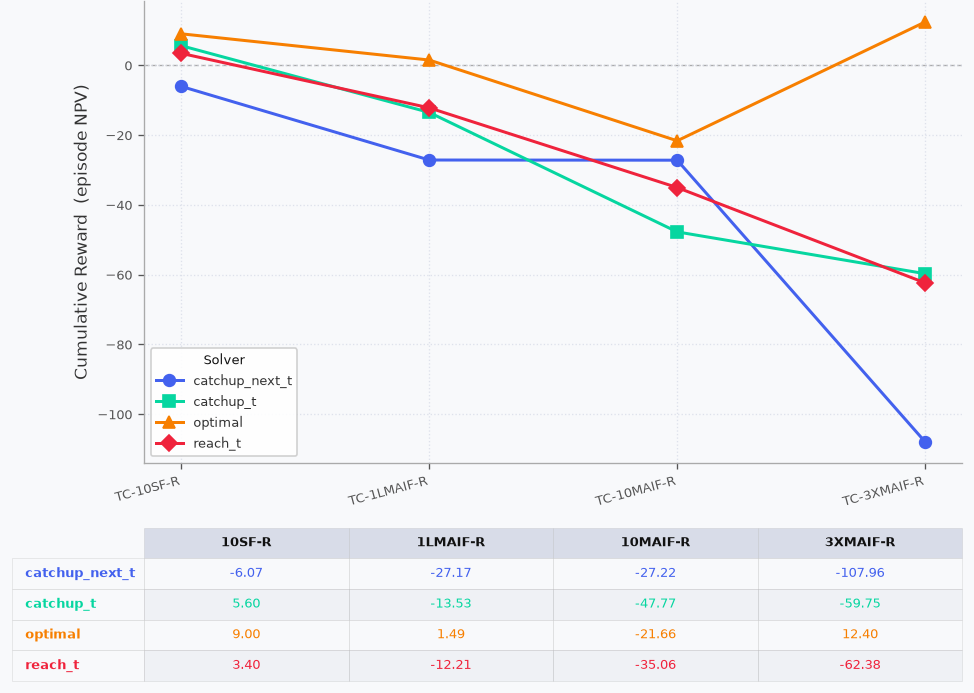
\includegraphics[width=\textwidth]{figures/gap_plot.png}
    \caption{Cumulative episode NPV (reward) for three greedy heuristics and
    the full-information optimum across four benchmark configurations of
    increasing portfolio complexity. The widening gap as complexity grows
    motivates the use of learned allocation policies.}
    \label{fig:gap_plot}
\end{figure}

% ------------------------------------------------------------
\subsection{Contributions and Paper Organisation}
\label{subsec:organisation}
% ------------------------------------------------------------

The contributions of this paper are threefold.

\begin{enumerate}[leftmargin=*, label=\textbf{C\arabic*.}]

    \item \textbf{Environment.} A configurable, Gymnasium-compatible CMDP
    environment encoding the full FIDIC contract cash-flow cycle: advance
    payment and progressive recovery, progress-weighted milestone payments,
    retention withholding and release, treasury-draw interest on negative
    cash balances that persists until the portfolio returns to surplus, and a
    two-condition termination gate with a project-specific cure-period counter.
    All environment parameters are specified through a configuration dictionary
    whose entries are probability distributions, allowing practitioners in any
    project-based sector---construction, IT, R\&D, or otherwise---to instantiate
    domain-specific environments by fitting those distributions to historical
    company data.
    Gymnasium API compliance is verified via \texttt{tests/gym\_test.py} across
    51 checks in 10 test sections; the full compatibility certificate is
    reproduced in Appendix~\ref{app:gym_certificate}.
    The environment ships with a SQLite audit ledger that records every
    allocation, cash-flow event, and breach flag at each episode step,
    making learned policy behaviour fully interpretable.

    \item \textbf{MDP Formulation.} A formal specification of the
    portfolio budgeting problem as a CMDP: state space, action space, transition
    dynamics, reward signal, and the observation vector presented in closed form.

    \item \textbf{Baseline Benchmark and Optimality Gap.} Three deterministic
    greedy heuristics evaluated against a full-information optimum across four
    benchmark configurations, producing a quantified optimality gap that grows
    monotonically with portfolio complexity and establishes the performance
    target for future reinforcement learning agents.

\end{enumerate}

Section~\ref{sec:literature} reviews the relevant literature across four
streams: project management foundations, portfolio management and selection,
PPM budgeting and cash-flow modelling, and reinforcement learning for
sequential resource allocation.
Section~\ref{sec:problem} develops the MDP formulation formally.
Section~\ref{sec:evaluation} presents the benchmark evaluation: three
deterministic greedy heuristics and a full-information optimum across four
portfolio configurations, quantifying the optimality gap that motivates
learned agents.
Training RL agents on the environment and evaluating them against a formal
Linear Programming bound are left as the natural next step, addressed in
subsequent work.